\documentclass[conference]{IEEEtran}
\IEEEoverridecommandlockouts
\newcommand\tab[1][0.5cm]{\hspace*{#1}}
\usepackage{amsmath,amssymb,amsfonts}
\usepackage{algorithmic}
\usepackage{graphicx}
\usepackage{listings}
\usepackage{textcomp}
\usepackage{xcolor}
\usepackage{url}
\usepackage[style=ieee,backend=biber]{biblatex}
\usepackage{float}
\usepackage[T1]{fontenc}
\usepackage[scaled]{beramono}
\addbibresource{ref.bib}

\usepackage{color}
\definecolor{bluekeywords}{rgb}{0.13,0.13,1}
\definecolor{greencomments}{rgb}{0,0.5,0}
\definecolor{redstrings}{rgb}{0.9,0,0}
%\lstset { %
%	language=C,
%	backgroundcolor=\color{black!5}, 
%	basicstyle=\footnotesize,
%}
\lstset{language=C,
	showspaces=false,
	showtabs=false,
	breaklines=true,
	showstringspaces=false,
	breakatwhitespace=true,
	escapeinside={(*@}{@*)},
	commentstyle=\color{greencomments},
	keywordstyle=\color{bluekeywords},
	stringstyle=\color{redstrings},
	basicstyle=\ttfamily
}
    
\begin{document}

\title{CoE 135: Lab 7 Documentation (Memory)\\
}

\author{\IEEEauthorblockN{Salmon, Paulino III I. }
	\IEEEauthorblockA{\textit{2015-11557}\\
	paulino.salmon@eee.upd.edu.ph}}		
\maketitle

\section{Properties of kmalloc() (50 pts)}
\begin{enumerate}
\item Does kmalloc() always allocate memory sizes in powers of two? \\
\tab To answer this, I created a for loop in my kernel module that would continuously just allocate and free memory used by kmalloc() at a maximum value of 255. This counter is to be plugged in the code line: \textbf{ptr = kmalloc(i, GFP\_KERNEL);}
\begin{lstlisting}
// #1
unsigned int i;
for(i = 0; i < 255; i++) {
	ptr = kmalloc(i, GFP_KERNEL);
	printk(KERN_INFO "I got: %zu bytes of memory. I is: %d\n", ksize(ptr), i);
	kfree(ptr);
}
\end{lstlisting}
\tab Running this kernel module in \textit{dmesg}, it shows that the allocated bytes of memory are \textbf{not always} in powers of two (See 96 bytes and 192 bytes below).
\begin{center}
	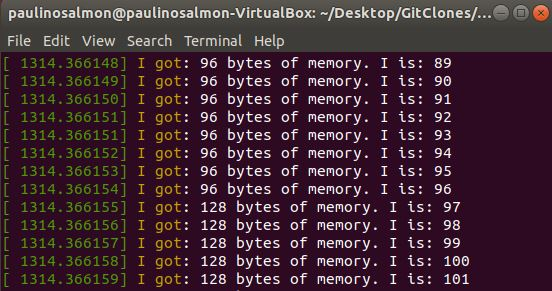
\includegraphics[width=8.5cm, height=4.5cm]{memory1.JPG}
\end{center}
\begin{center}
	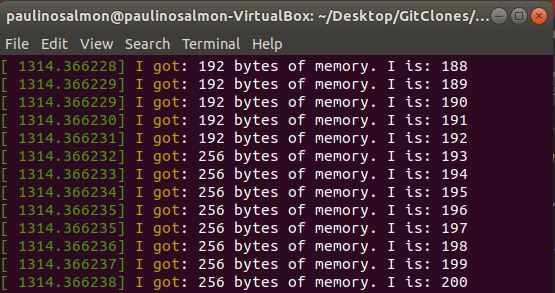
\includegraphics[width=8.5cm, height=4.5cm]{memory2.JPG}
\end{center}
\tab Page sizes are normally in powers of two, but the system allocates usually a little bit more than what is asked for as according to Stack Overflow User \textcite{kmalloc}. \\

%%%%%%%%%%%%%%%%%%%%%%%%%%%%%%%%%%%%%%%%

\item What is the minimum amount of memory kmalloc() can provide?

\tab Using the code snippet below and printing the kernel module in \textit{dmesg} afterwards:
	\begin{lstlisting}
// #2
printk(KERN_INFO "Minimum size is: %d bytes.\n", KMALLOC_MIN_SIZE);
	\end{lstlisting}
	\begin{center}
		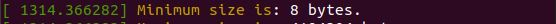
\includegraphics[width=8.5cm, height=0.3cm]{memory3.JPG}
	\end{center}
\tab Terminal output shows that the minimum amount of memory kmalloc() can provide is \textbf{8 bytes}. This KMALLOC\_MIN\_SIZE constant is defined in the slab.h header. \\
%%%%%%%%%%%%%%%%%%%%%%%%%%%%%%%%%%%%%%%%

\item What is the maximum amount of memory kmalloc() can provide?

\tab Using the code snippet below and printing the kernel module in \textit{dmesg} afterwards:
\begin{lstlisting}
// #3
printk(KERN_INFO "Maximum size is: %ld bytes.\n", KMALLOC_MAX_SIZE);
\end{lstlisting}
\begin{center}
	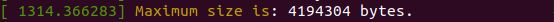
\includegraphics[width=8.5cm, height=0.3cm]{memory4.JPG}
\end{center}
\tab Terminal output shows that the minimum amount of memory kmalloc() can provide is \textbf{4194304 bytes}. This KMALLOC\_MAX\_SIZE constant is defined in the slab.h header. \\
%%%%%%%%%%%%%%%%%%%%%%%%%%%%%%%%%%%%%%%%

\item Is the memory given to you by kmalloc() physically contiguous? \\
\tab As per Stack Overflow Users \textcite{kmallocvsvmalloc}, the kmalloc() function guarantees that the pages are both physically and virtually contiguous, although, contiguity for kmalloc() may fail if the order of allocation is already very high.
\end{enumerate}

%%%%%%%%%%%%%%%%%%%%%%%%%%%%%%%%%%%%%%%%
\section{Memory and Paging (50 pts)}
\begin{enumerate}
\item Determine the value of the Page Size in the system you are currently using. 

\tab Using the code snippet below and printing the kernel module in \textit{dmesg} afterwards:
\begin{lstlisting}
// #1
printk(KERN_INFO "Page size is: %ld bytes.\n", PAGE_SIZE);
\end{lstlisting}
\begin{center}
	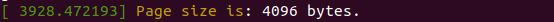
\includegraphics[width=8cm, height=0.3cm]{memory5.JPG}
\end{center}
\tab Terminal output shows that the value of the page size is \textbf{4096 bytes}. This PAGE\_SIZE constant is also already defined in one of the linux headers. \\

%%%%%%%%%%%%%%%%%%%%%%%%%%%%%%%%%%%%%%%%

\item Determine the start of the HIGHMEM region of your memory. Clearly state the
architecture used by your machine when answering this problem. 

\tab Invoking the \textit{hostnamectl} terminal command, it shows that my system is of the 64-bit architecture.

\begin{center}
	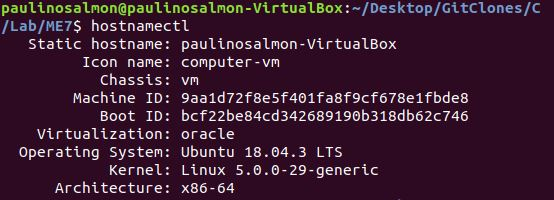
\includegraphics[width=8cm, height=3cm]{memory6.JPG}
\end{center}

\tab 64-bit processors can directly access $2^{64}$ bytes of memory. As per Users \textcite{highmem}, the linux kernel splits these into the high memory (user space) and the low memory (kernel space). Compared to 32-bit machines in which the high memory address range starts at 0x00000000, high memory does not exist for 64-bit machines as it can access a huge memory of 16 EB, theoretically giving anyone more RAM than they ever need in the entire history of computing. \\

%%%%%%%%%%%%%%%%%%%%%%%%%%%%%%%%%%%%%%%% 

\item Determine if the memory given by vmalloc() is physically contiguous per page, and if
the memory given by vmalloc() is physically contiguous overall. 

\tab As per \textcite{kmallocvsvmalloc}, vmalloc() allocates memory that is virtually contiguous but not necessarily physically contiguous overall.
\begin{center}
	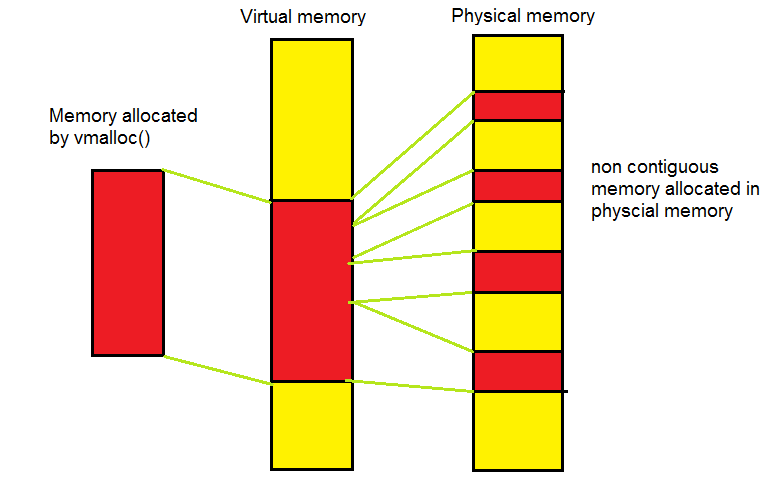
\includegraphics[width=8.5cm, height=6cm]{memory7.JPG}
\end{center}
%%%%%%%%%%%%%%%%%%%%%%%%%%%%%%%%%%%%%%%% 

\item Determine if the memory given by vmalloc() in the HIGHMEM region corresponds to
a physical memory address.

\tab A memory allocated by vmalloc() has a virtual address, but this may not be necessarily mapped directly to a physical address. The vmalloc() function only allocates contiguous virtual memory. This entire chuck may be fragmented when it comes to physical memory address translation, as show in the previous image.
\end{enumerate}
%%%%%%%%%%%%%%%%%%%%%%%%%%%%%%%%%%%%%%%%%%%%%%
\printbibliography
\end{document}